
\subsection{Path Tracking}\label{subsec:prob2.3}

\begin{wrapfigure}{r}{0.5 \textwidth}
\vspace{-15mm}
\centering
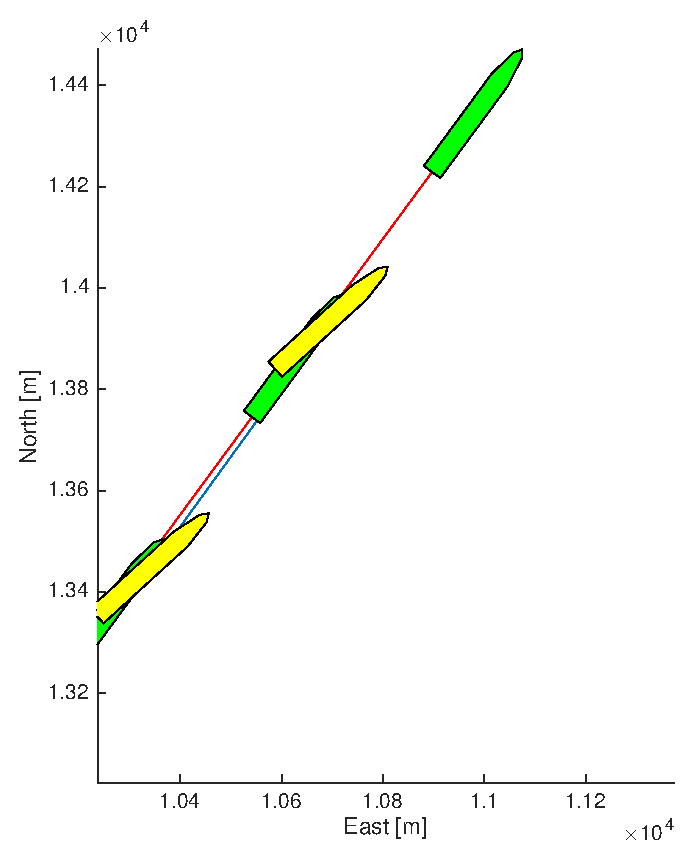
\includegraphics[height=0.5 \textheight]{task2.7/Task2_7-1-zoom}
\caption{Target tracking (zoom)}
\label{fig:2.7-tracking-zoom}
\vspace{-20mm}
\end{wrapfigure}
We want to follow a target with constant speed and course made up by the two first waypoints. This is essentially the same as path following with only one active segment, and a speed controller ensuring that we intercept the target and keep a constant distance from it. The heading and speed controller in use is the same as in section \ref{subsec:prob2.2}, and we have added a computation of $\tilde{\mathbf{p}} = \mathbf{p} - \mathbf{ p}_t$ which is a two dimensional vector from the target to our position. This vector is used by the speed guidance block to determine the distance to the target, and calculate the desired speed vector.
\begin{equation}
\begin{split}
\mathbf{v}_d &= \mathbf{v}_t + \mathbf{v}_a \\
\mathbf{v}_a &= -\kappa \frac{ \tilde{ \mathbf{p} } } { || \tilde{ \mathbf{p} } ||} \\
\kappa &= U_{a,max} \frac{ || \tilde{ \mathbf{p} } || } { \sqrt{ ( \tilde{ \mathbf{p}} )^T  \tilde{ \mathbf{p} } + \Delta_s^2 }}
\end{split}
\end{equation}
Where $U_{a,max}$ and $\Delta_s^2$ are design parameters describing the maximum relative velocity between the intercepting ship and target and transient interceptor-target rendezvous behavior respectively. 
\begin{figure}[h]
\begin{center}
 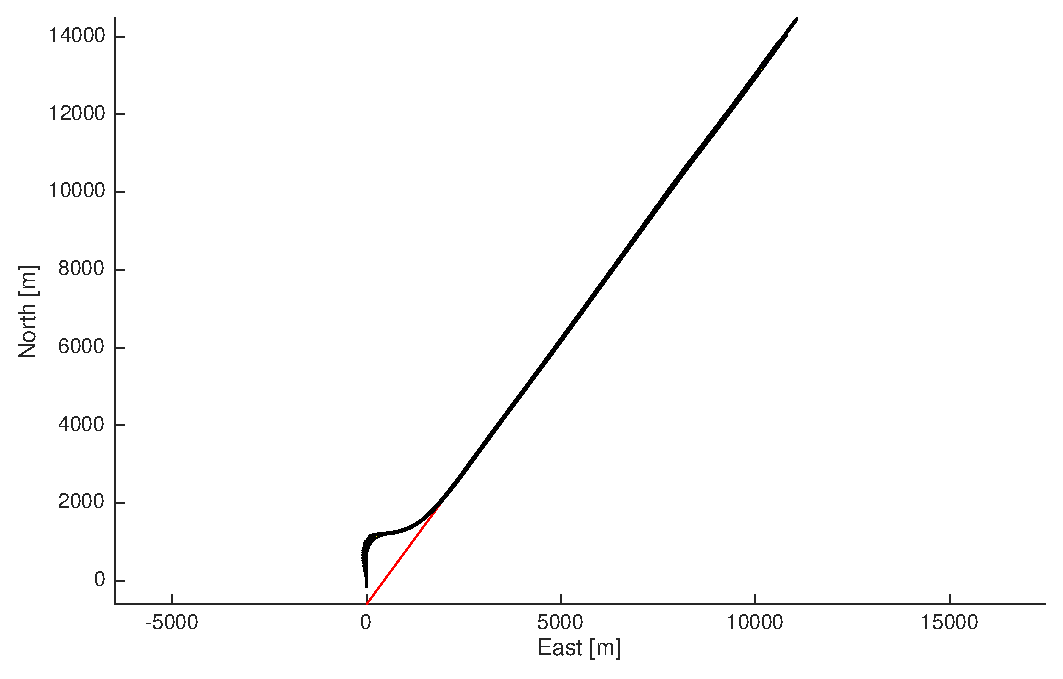
\includegraphics[height=0.4 \textheight]{task2.7/Task2_7-1}
\caption{Target tracking}
\label{fig:2.7-tracking}
\end{center}
\end{figure}

\begin{figure}[h]
\begin{center}
 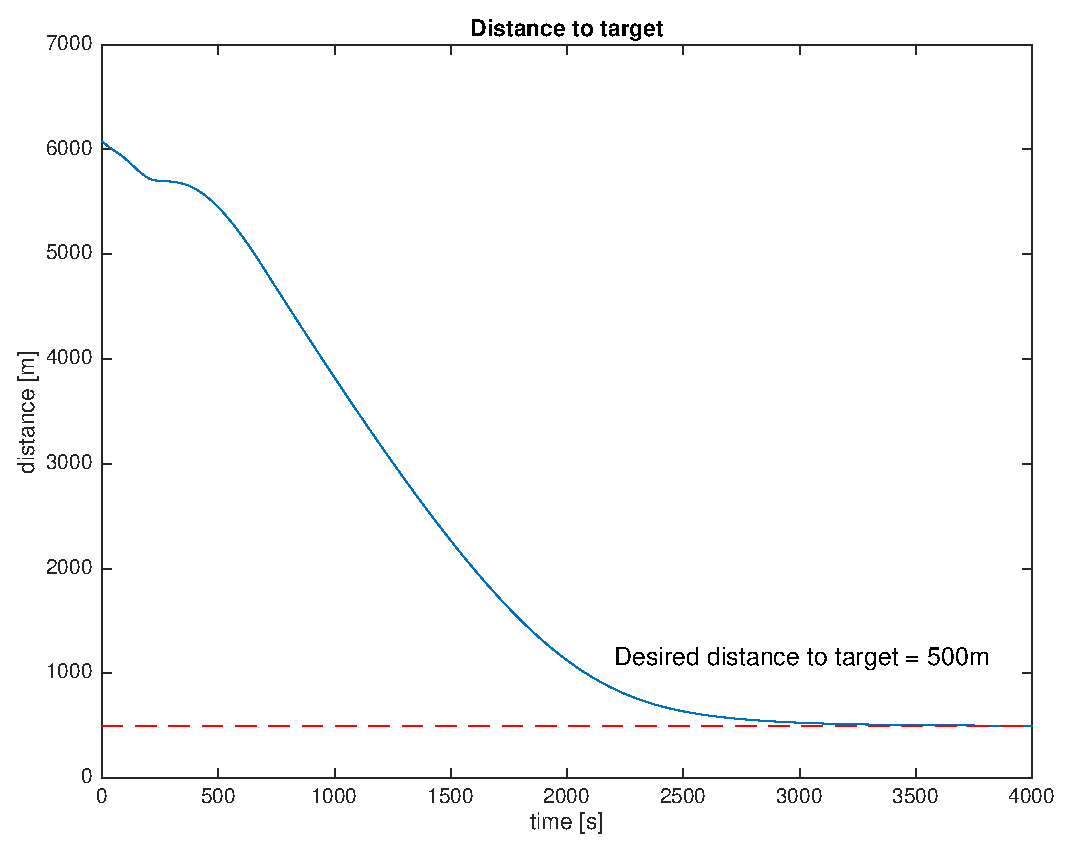
\includegraphics[height=0.4 \textheight]{task2.7/Task2_7-2}
\caption{Interception of target}
\label{fig:2.7-D2T}
\end{center}
\end{figure}